%%%%%%%%%%%%%%%%%%%%%%%%%%%%%%%%%%%%%%%%%%%%%%%%%%%%%%%%%%%%%%%
%
% Welcome to Overleaf --- just edit your LaTeX on the left,
% and we'll compile it for you on the right. If you open the
% 'Share' menu, you can invite other users to edit at the same
% time. See www.overleaf.com/learn for more info. Enjoy!
%
%%%%%%%%%%%%%%%%%%%%%%%%%%%%%%%%%%%%%%%%%%%%%%%%%%%%%%%%%%%%%%%


% Inbuilt themes in beamer
\documentclass{beamer}

% Theme choice:
\usetheme{CambridgeUS}
\usepackage{amsmath}

\usepackage{array}
\newcolumntype{P}[1]{>{\centering\arraybackslash}p{#1}}

% Title page details: 
\title{AI1110: Probability and Random Variables}
\subtitle{Assignment 6}
\author{Rishit D (cs21btech11053)}
\institute{IIT Hyderabad}
\date{\today}


\begin{document}

% Title page frame
\begin{frame}
    \titlepage 
\end{frame}

% Outline frame
\begin{frame}{Outline}
    \tableofcontents
\end{frame}

% Problem
\section{Problem}

\begin{frame}{Assignment 6}
  \frametitle{Problem}
  Find the probability distribution of
  \begin{enumerate}
    \item number of heads in two tosses of a coin.
    \item number of tails in the simultaneous tosses of three coins.
    \item number of heads in four tosses of a coin.
  \end{enumerate}
\end{frame}

% Solution
\section{Solution}
\subsection{Binomial Distribution}

%Defining Random Variables
\begin{frame}
  \frametitle{Binomial Distributions}
  Take a Bernoulli trial with parameter $p$ represented by random variable $X$, where probability that $X = 1$ is $p$ and $X = 0$ is $1-p$. If this trial is repeated $n$ times, we obtain a binomial distribution.
  The probability that $X = i$, that is, $X = 1$ occurs exactly $i$ times out of $n$ trials is given by
  \begin{block}{Binomial Distribution for $X = i$}
    \begin{align}
      \Pr(X = i) = \binom{n}{i} \times p^i \times (1-p)^{n-i}
      \label{eq:BinomProb}
    \end{align}
  \end{block}
\end{frame}


%Heads in 2 tosses
\subsection{Part 1}
\begin{frame}
  \frametitle{Number of \emph{heads} in 2 tosses of a coin}
  Assume $X_1$ to be a random variable representing the number of \emph{heads} in $n = 2$ trials. Using
  \eqref{eq:BinomProb}
  we can define the probability mass function of the random variable $X_1$ as follows
  \begin{align}
    \Pr(X_1 = k) = 
    \begin{cases}
      \frac{1}{4}, & k = 0 \\
      \frac{1}{2}, & k = 1 \\
      \frac{1}{4}, & k = 2 \\
      0, & \text{otherwise}
    \end{cases}
    \label{eq:Pmf1}
  \end{align}

  Refer next slide for graph
  \eqref{fig:pmfGraph1}
\end{frame}

\begin{frame}
  \frametitle{Graph for Part 1}
  \begin{figure}[!ht]
    \centering
    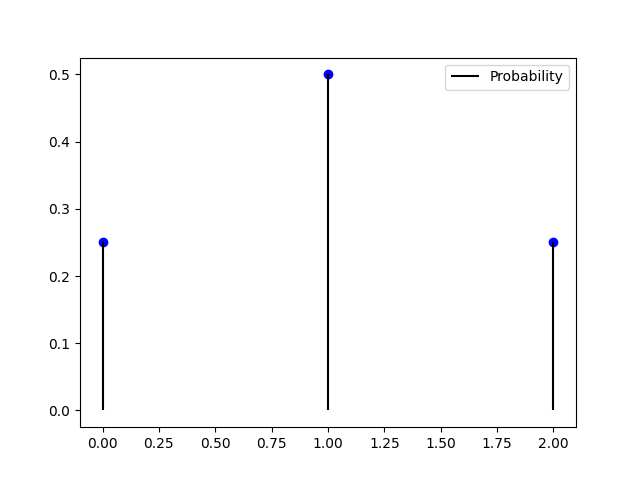
\includegraphics[width=0.5\columnwidth]{../Figures/coin1.png}
    \caption{PMF for Part 1}
    \label{fig:pmfGraph1}
  \end{figure}
\end{frame}

%Tails in 3 tosses
\subsection{Part 2}
\begin{frame}
  \frametitle{Number of \emph{tails} in simultaneous tosses of 3 coins}
  This is the same as tossing a coin 3 times. Assume $X_2$ to be a random variable representing the number of \emph{tails} in $n = 3$ trials. Using
  \eqref{eq:BinomProb}
  we can define the probability mass function of the random variable $X_2$ as follows
  \begin{align}
    \Pr(X_2 = k) = 
    \begin{cases}
      \frac{1}{8}, & k = 0 \\
      \frac{3}{8}, & k = 1 \\
      \frac{3}{8}, & k = 2 \\
      \frac{1}{8}, & k = 3 \\
      0, & \text{otherwise}
    \end{cases}
    \label{eq:Pmf2}
  \end{align}

  Refer next slide for graph
  \eqref{fig:pmfGraph2}
\end{frame}

\begin{frame}
  \frametitle{Graph for Part 2}
  \begin{figure}[!ht]
    \centering
    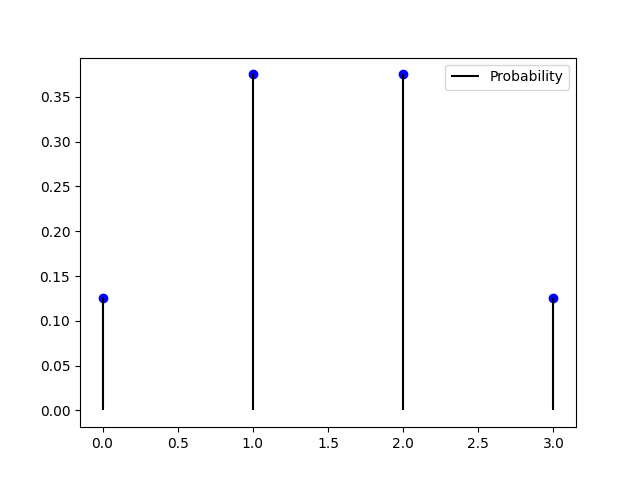
\includegraphics[width=0.5\columnwidth]{../Figures/coin2.png}
    \caption{PMF for Part 2}
    \label{fig:pmfGraph2}
  \end{figure}
\end{frame}

%Heads in 4 tosses
\subsection{Part 3}
\begin{frame}
  \frametitle{Number of \emph{heads} in 4 tosses of a coin}
  Assume $X_3$ to be a random variable representing the number of \emph{heads} in $n = 2$ trials. Using
  \eqref{eq:BinomProb}
  we can define the probability mass function of the random variable $X_3$ as follows
  \begin{align}
    \Pr(X_3 = k) = 
    \begin{cases}
      \frac{1}{16}, & k = 0 \\
      \frac{1}{4}, & k = 1 \\
      \frac{3}{8}, & k = 2 \\
      \frac{1}{4}, & k = 3 \\
      \frac{1}{16}, & k = 4 \\
      0, & \text{otherwise}
    \end{cases}
    \label{eq:Pmf3}
  \end{align}

  Refer next slide for graph
  \eqref{fig:pmfGraph3}
\end{frame}

\begin{frame}
  \frametitle{Graph for Part 3}
  \begin{figure}[!ht]
    \centering
    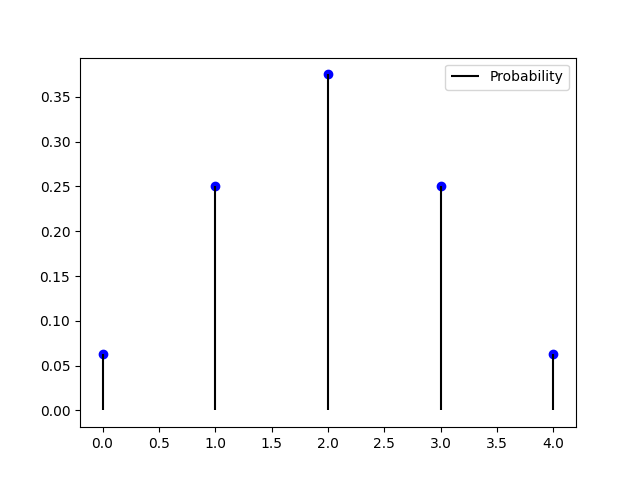
\includegraphics[width=0.5\columnwidth]{../Figures/coin3.png}
    \caption{PMF for Part 3}
    \label{fig:pmfGraph3}
  \end{figure}
\end{frame}

\end{document}
